% !TEX root = main.tex
\section{Overview}

This application is a game called `Elemental Slots'.
It is based on a slot machine game where you spend money and get rewards based on your luck.
Every roll is a random 6-digit number where it will be tested through each \emph{achievement} and give handout if the condition is met.

\begin{tabbing}
    \hspace*{2.2cm} \= \kill
    Repository \> \url{https://github.com/2110215-ProgMeth/cp-project-2025-2-sanelarbkoi} \\
    JavaDoc \> \url{https://paristp.github.io/2110215_javadoc/}
\end{tabbing}

\subsection{Menu}

When you first open the game, you will be welcomed with this menu screen.
A Vietnamese music will start playing in the background.
There are 4 buttons you can press; \textsc{start, settings, leaderboard} and \textsc{exit}.

\begin{figure}[H]
    \centering
    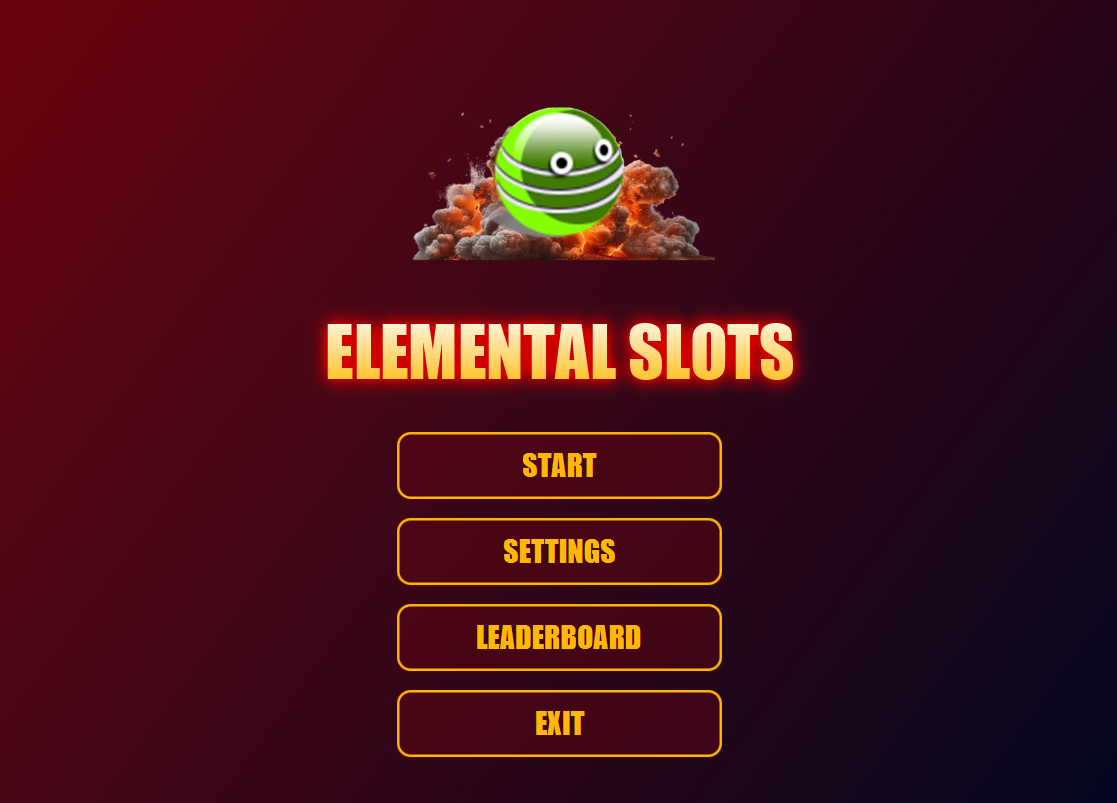
\includegraphics[scale=0.36]{Images/menu.png}
    \caption{Menu screen}
\end{figure}

If you press \textsc{start}, you will see this alert.
You can type your name into the field and press \textsc{ok} to log in.

\begin{figure}[H]
    \centering
    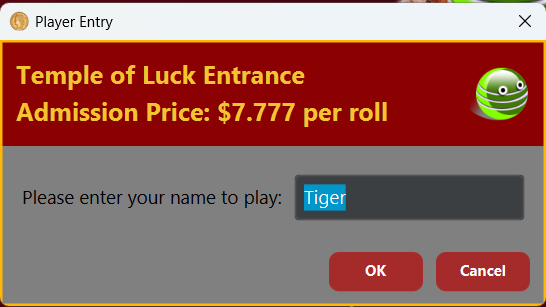
\includegraphics[scale=0.6]{Images/playerEntry.png}
    \caption{Name input alert}
\end{figure}

If you try to put in an empty name however, you will get this warning alert.
You will have to type your name again to get into the game.

\begin{figure}[H]
    \centering
    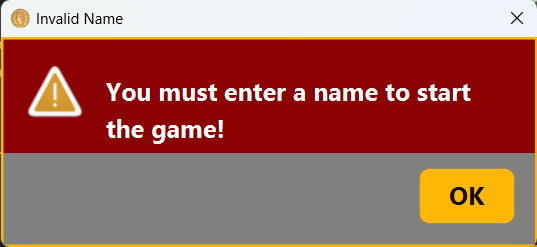
\includegraphics[scale=0.61]{Images/invalidName.png}
    \caption{Invalid name alert}
\end{figure}

\subsection{Settings}

If you press \textsc{settings}, you will open settings page.
Here, you can use these sliders to adjust the volume of game song and sound effects.
You can go back to \emph{menu screen} by hitting \textsc{back}.

\begin{figure}[H]
    \centering
    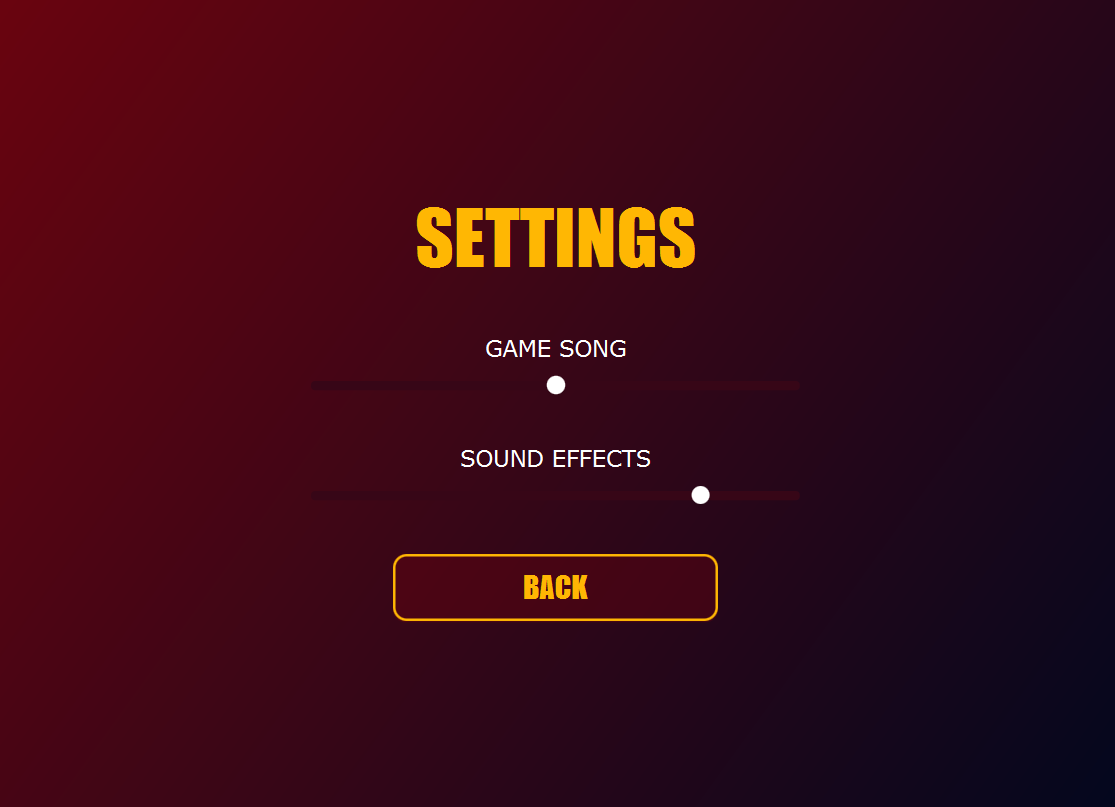
\includegraphics[scale=0.36]{Images/settings.png}
    \caption{Setting page}
\end{figure}

\subsection{Leaderboard}

If you press \textsc{leaderboard}, you will open temple leaderboard page.
Initially it won't have any data but if after some people have played, their stats will be shown here.

\begin{figure}[H]
    \centering
    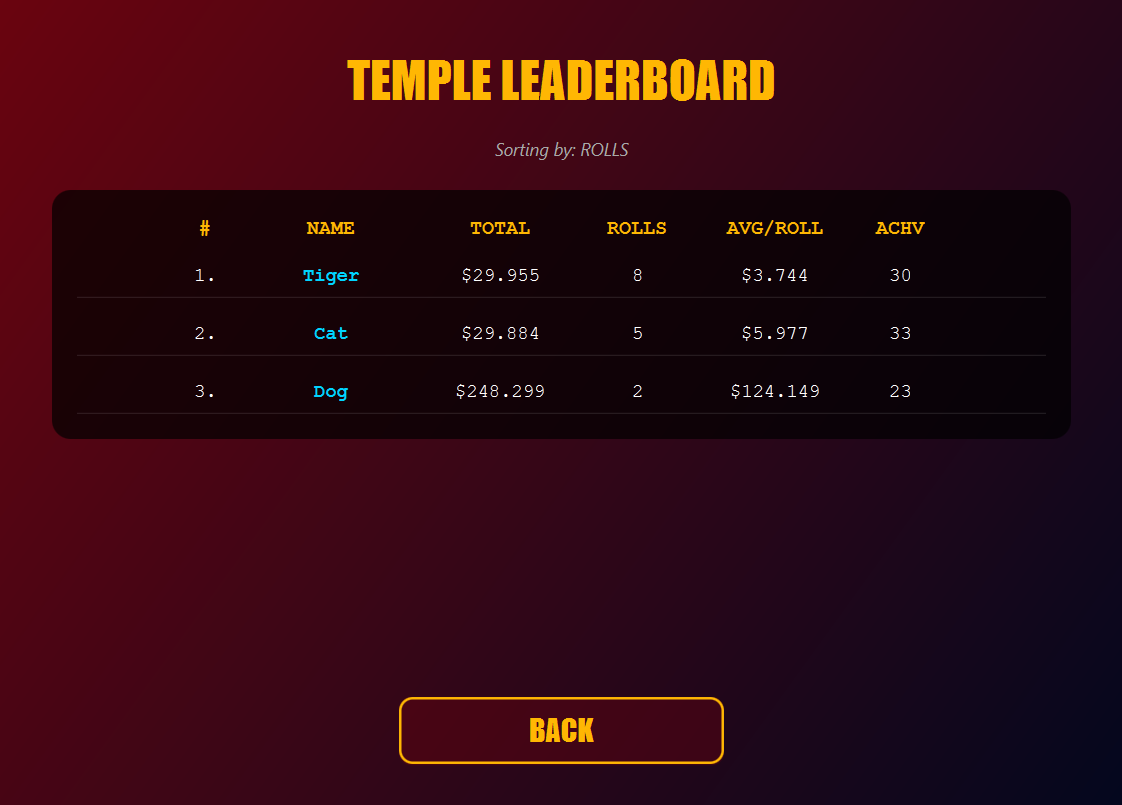
\includegraphics[scale=0.36]{Images/leaderboard.png}
    \caption{Leaderboard screen}
\end{figure}

You can press on each column to change the sorting condition.
If you click on a player's name, you will open their \emph{badge collection screen}.

\subsection{Badge Collection}

This is a collection page that shows all achievements that a player has gained.
Unlocked badges will be shown in gray `?'.
There are 138 badges in total from 6 rarities.

\begin{figure}[H]
    \centering
    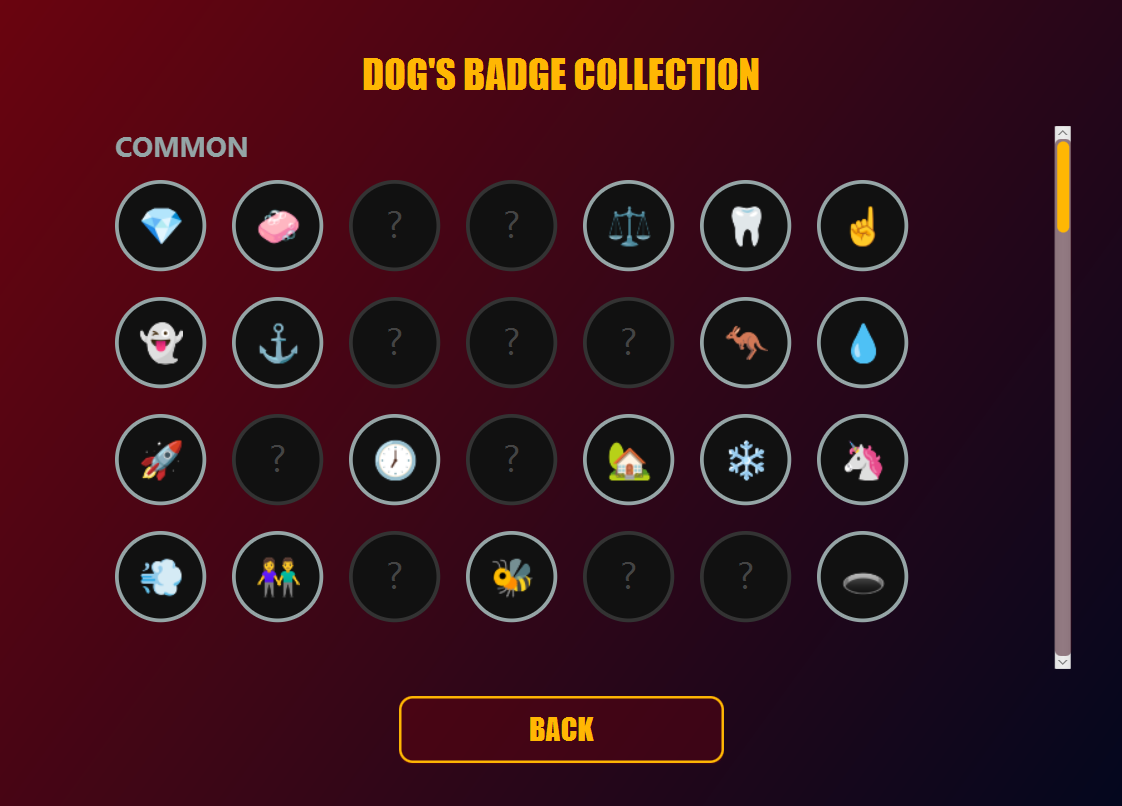
\includegraphics[scale=0.36]{Images/collection.png}
    \caption{Collection}
\end{figure}

By clicking on a badge, it will show this pop-up screen.
It contains player's record on getting this achievement.

\begin{figure}[H]
    \centering
    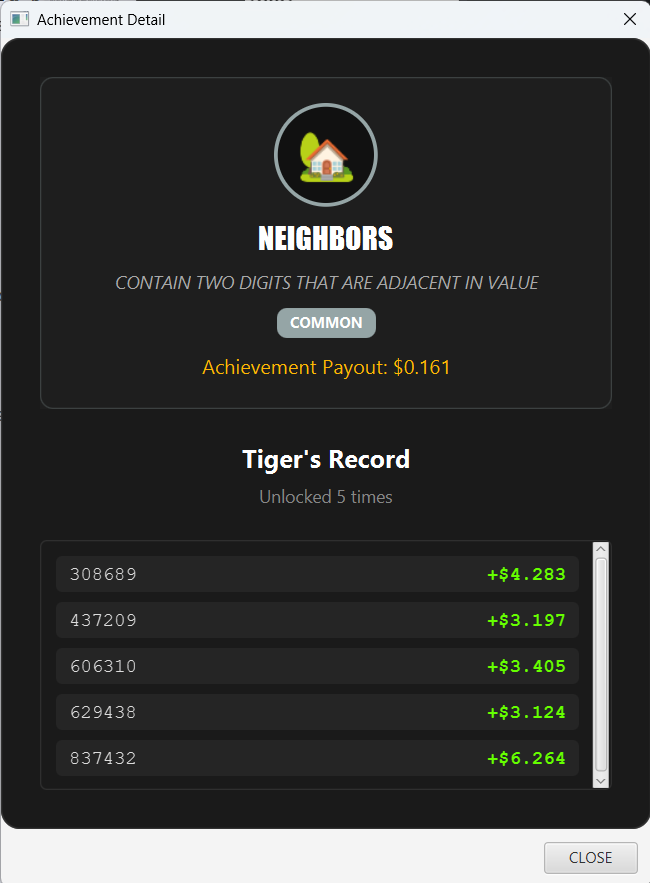
\includegraphics[scale=0.36]{Images/achievementDetail.png}
    \caption{Collection}
\end{figure}


\subsection{Loading Screen}

If you are logging in for the first time, it will open this loading screen while the system is calibrating slot machine's stats.
Every new player gets \$200 to start.
If done, it will open \emph{game screen}.

\begin{figure}[H]
    \centering
    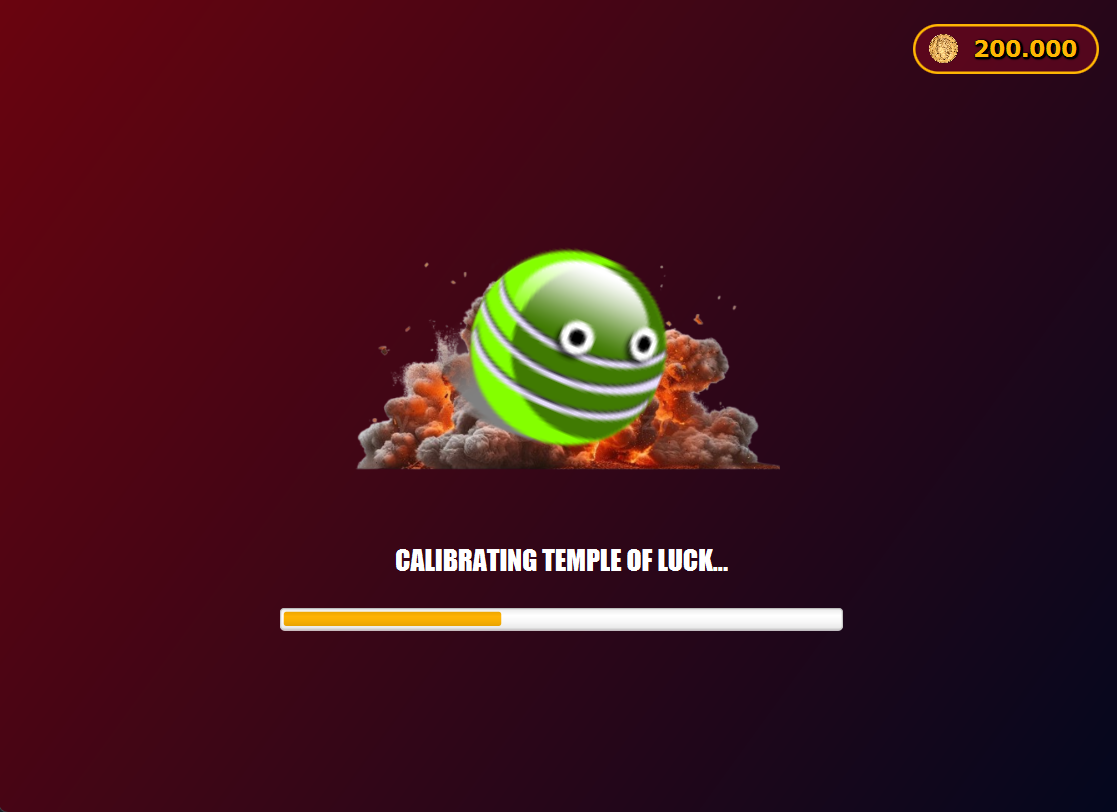
\includegraphics[scale=0.36]{Images/loading.png}
    \caption{Loading screen}
\end{figure}

\subsection{Game Screen}

This screen is where the slot machine is located.
You can play by clicking \textsc{roll}.
It costs \$7.777 and will roll a random number.

\begin{figure}[H]
    \centering
    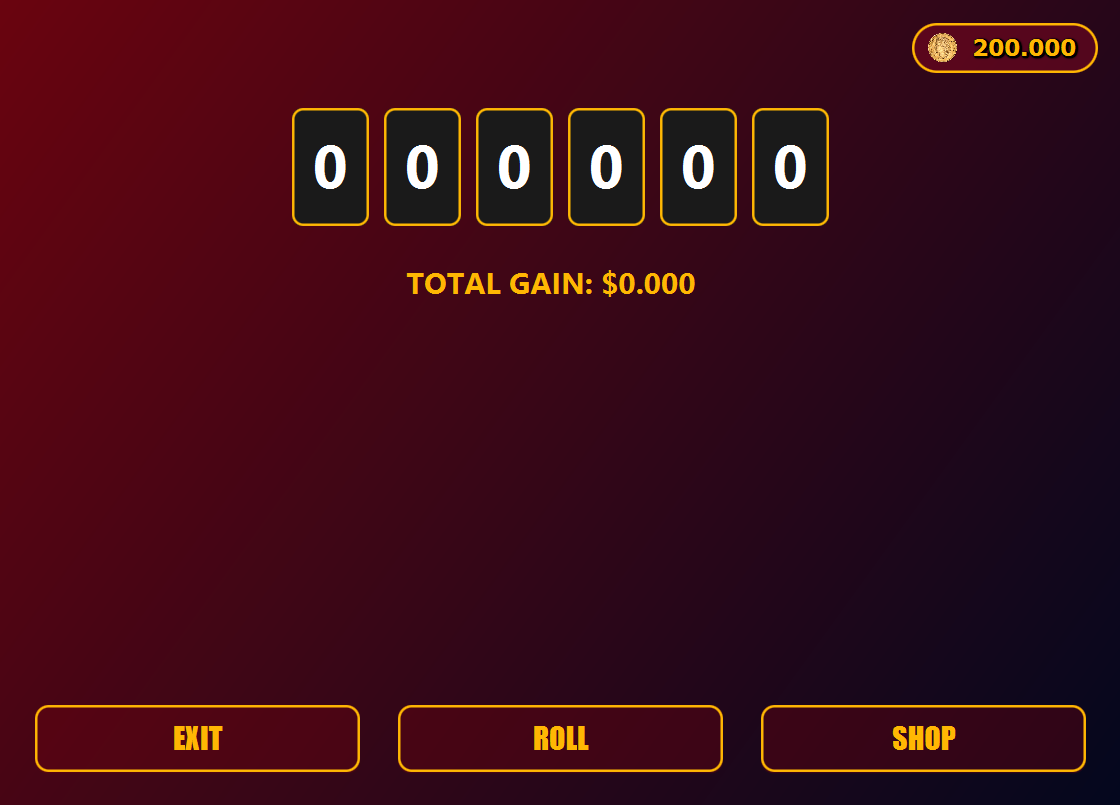
\includegraphics[scale=0.36]{Images/game0.png}
    \caption{Initial game screen}
\end{figure}

Then, every achievement which the roll satisfies its condition will appear one-by-one in the middle.
For example, if your roll is `410497', it will satisfy the `Prime' achievement because it is a prime number.

When an achievement box shows up, it will reward you with its value based on how rare it is to get.
You can read its name, condition, as well as its rarity.
If you get this achievement for the first time, it will have a red `new' tag.
You can also press \textsc{skip} to jump to the end.

\begin{figure}[H]
    \centering
    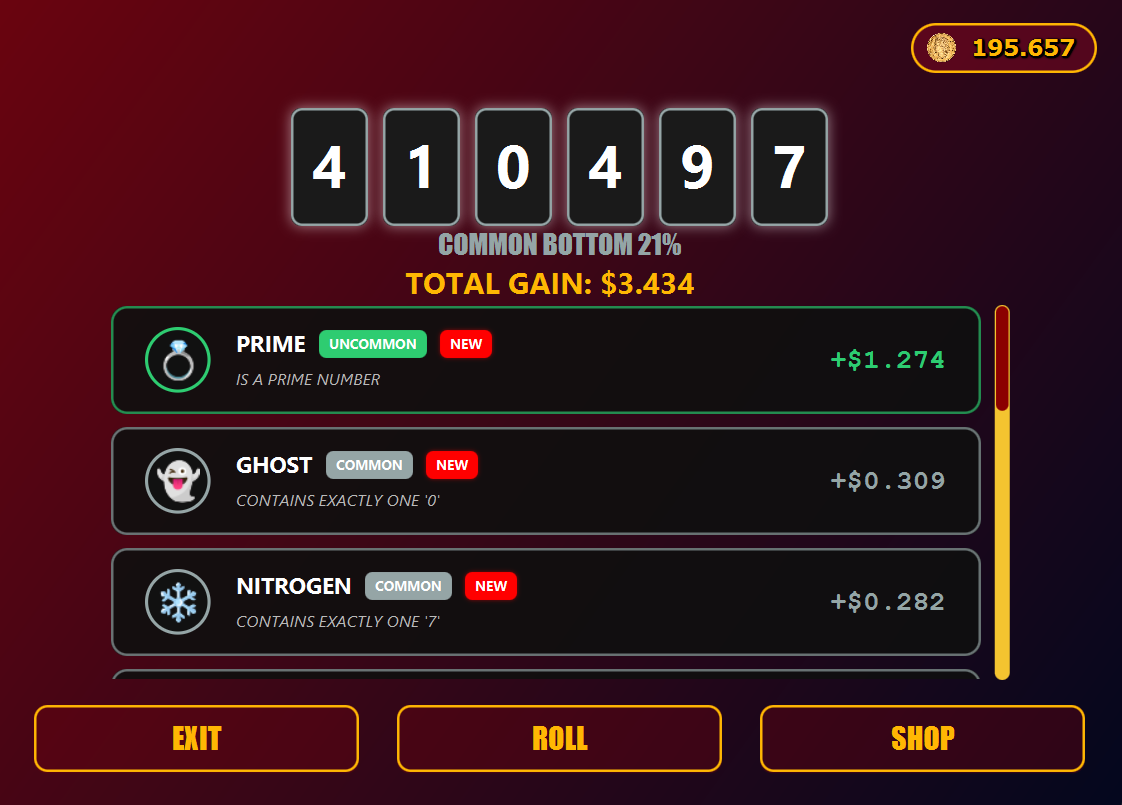
\includegraphics[scale=0.36]{Images/game1.png}
    \caption{Roll result}
\end{figure}

After every achievement showed up, the game will tell you the roll's percentile and your total money gained.
You can scroll through the details of the last roll.
Every roll is saved to player's history and updated to \emph{badge collection}.

\subsection{Booster Shop}

If you pressed \textsc{shop}, you will open booster shop.
You will see offers of boosts showing names, condition, price and amount you have.
Each boost will give you extra payout in percentages of your next roll if it satisfies the condition or else will be wasted.

\begin{figure}[H]
    \centering
    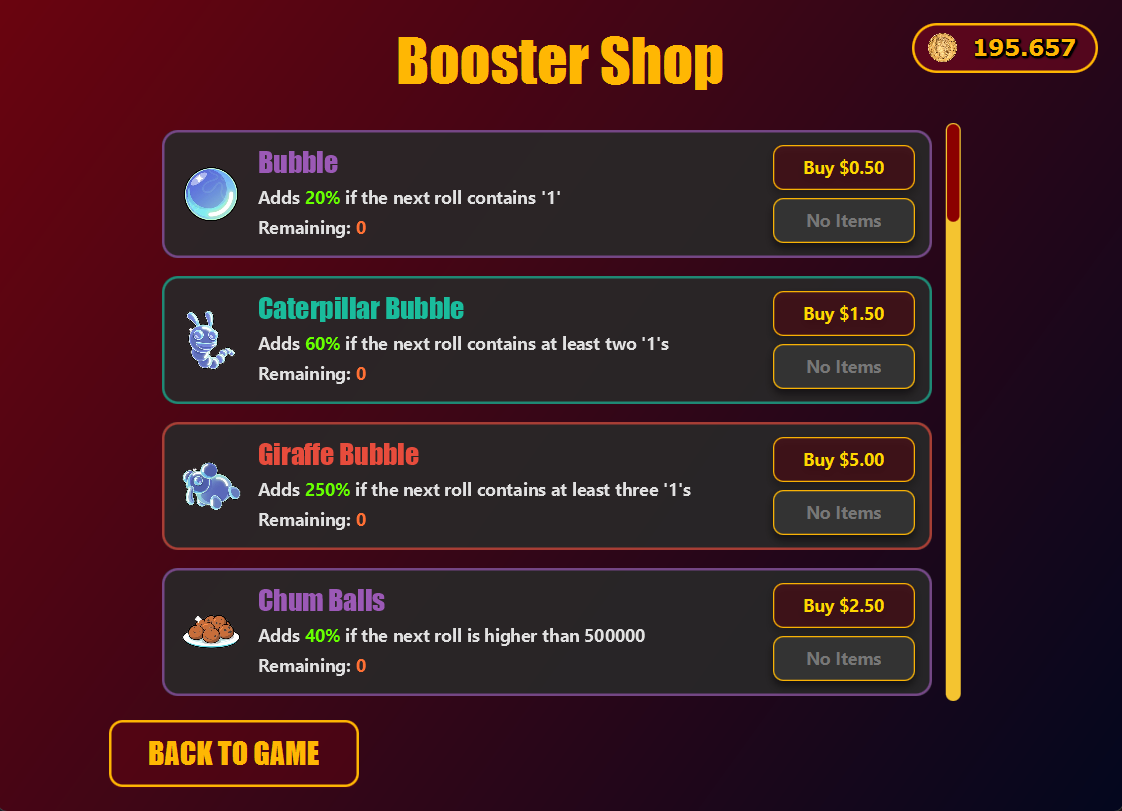
\includegraphics[scale=0.36]{Images/boosterShop0.png}
    \caption{Initial shop screen}
\end{figure}

You can click \textsc{buy} to pay money and add it to your inventory.
But if you don't have enough money, it will show `Can't buy' instead.
After you buy, you can click \textsc{activate} to add it to your next roll.

Once you press \textsc{activate}, it will take one of your stored item and add it to your active boost list.
If you press the same button again, it will \textsc{deactivate} that item and bring it back to your inventory.
Every active boosts will be used on the next roll.

\begin{figure}[H]
    \centering
    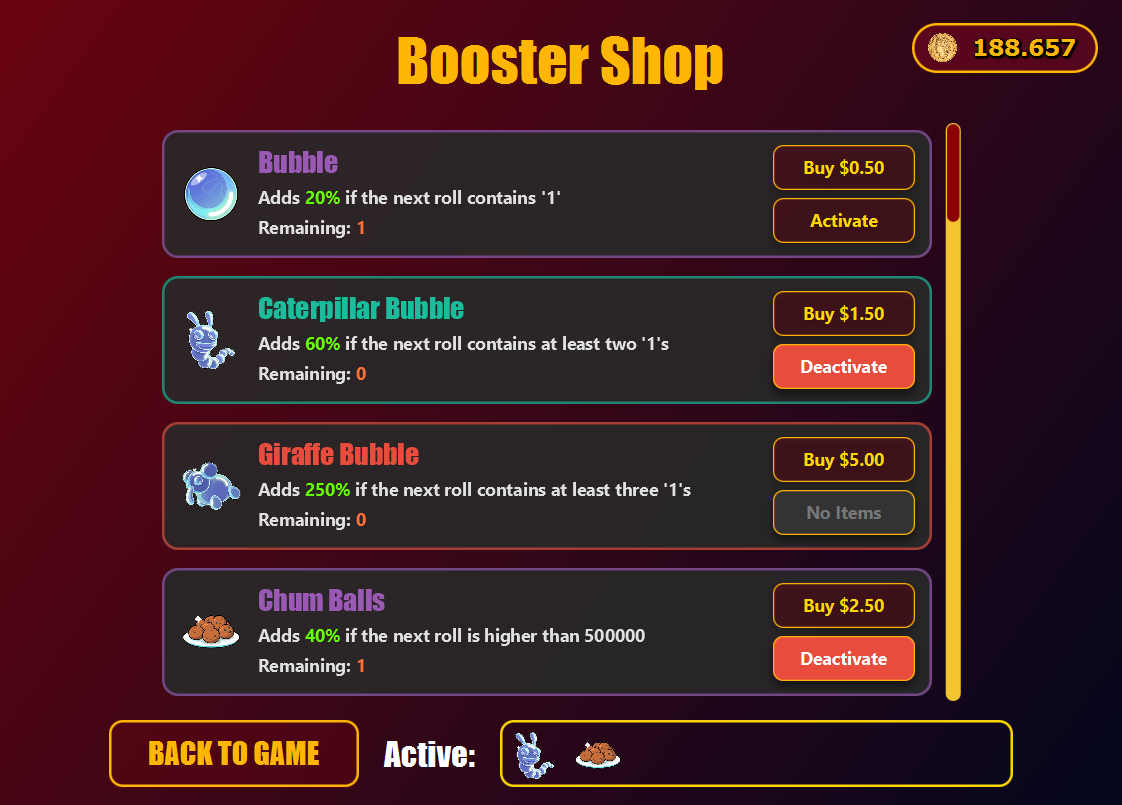
\includegraphics[scale=0.36]{Images/boosterShop1.png}
    \caption{Buying boosts}
\end{figure}

If you scroll down to bottom, you will see \textsc{buy all} and \textsc{activate all} buttons.
Pressing \textsc{buy all} will buy every boosts in the shop that you can afford except for \emph{Krusty Kash}.
Pressing \textsc{activate all} will activate (or deactivate) any boosts you have.

\begin{figure}[H]
    \centering
    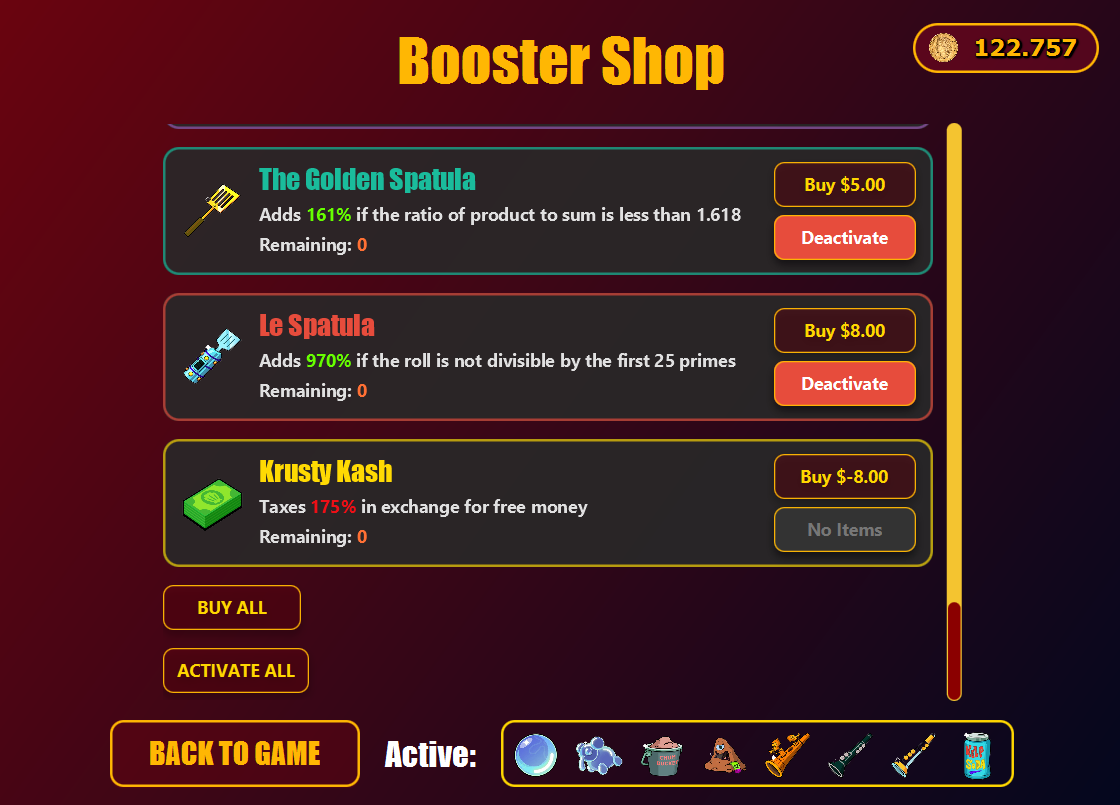
\includegraphics[scale=0.36]{Images/boosterShop2.png}
    \caption{Buy \& activate all}
\end{figure}

Krusty Kash is a special boost that it gives you free money but will take 175\% of payout on your next roll (kind of like a loan in case you fall short on money).
Once bought it will automatically be activated.

\subsection{Game Screen (cont.)}

If you play a game with boosts equipped and some of it does give rewards, it will show result next to `Total gain' text.
There will be an \textsc{i} icon that you can press to see more information of boost bonus.

\begin{figure}[H]
    \centering
    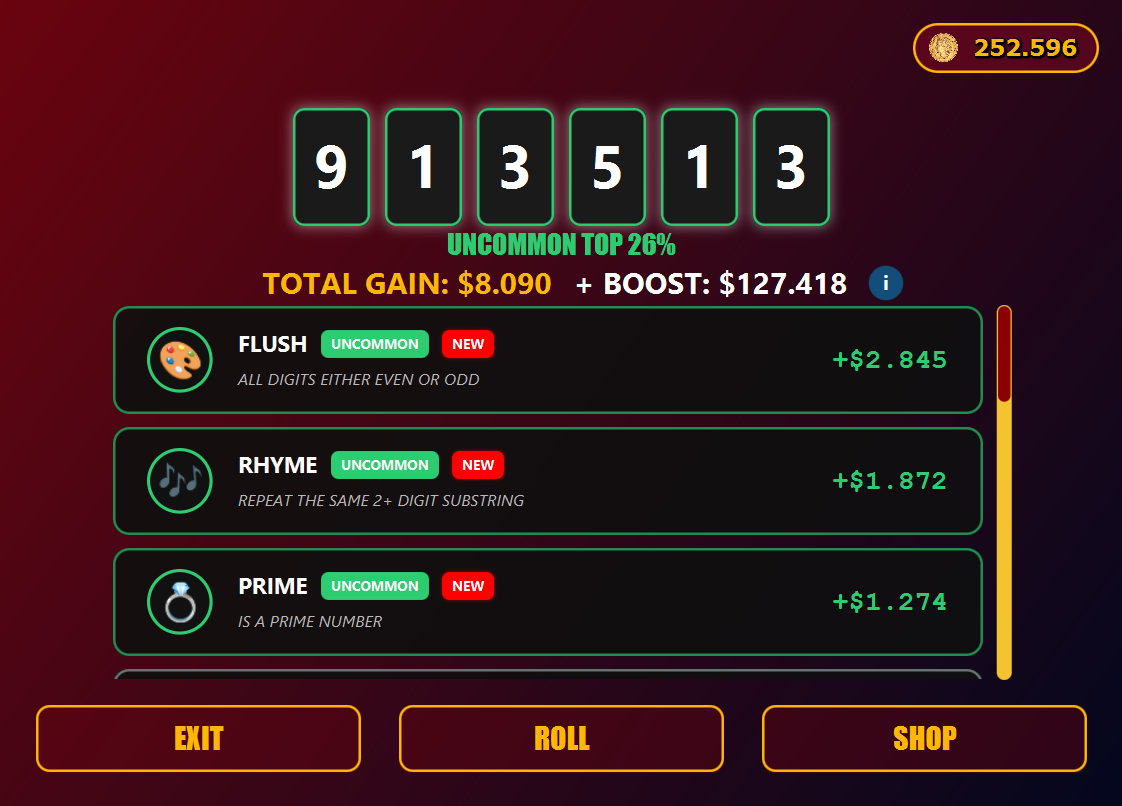
\includegraphics[scale=0.36]{Images/game2.png}
    \caption{Roll result with boost}
\end{figure}

\begin{figure}[H]
    \centering
    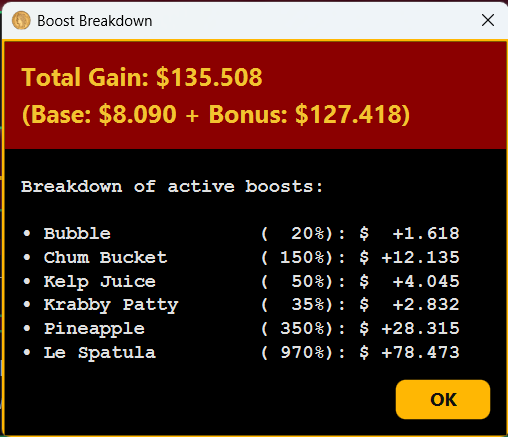
\includegraphics[scale=0.6]{Images/boostBreakdown.png}
    \caption{Boost breakdown alert}
\end{figure}

If you have less than \$7.777, you will have to borrow money from Krusty Kash (if you can) or you will get this message once you click \textsc{roll}.

\begin{figure}[H]
    \centering
    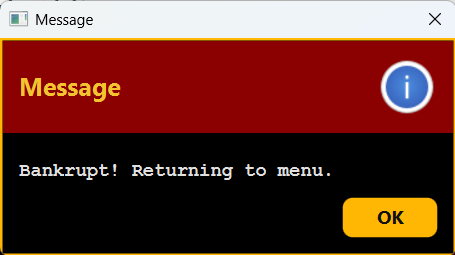
\includegraphics[scale=0.65]{Images/bankrupt.png}
    \caption{Bankrupt alert}
\end{figure}

You are bankrupt and will then be redirected to \emph{menu screen} and your player data will be removed from the game.
You can still create a new player with the same name but all past info will be removed.






